\section{Atom in a damped cavity}

In the previous sections we have discussed different parts of the system (fig. \ref{fig:before}) which we are going to combine in this section.

\begin{figure}[h!]
	\centering
	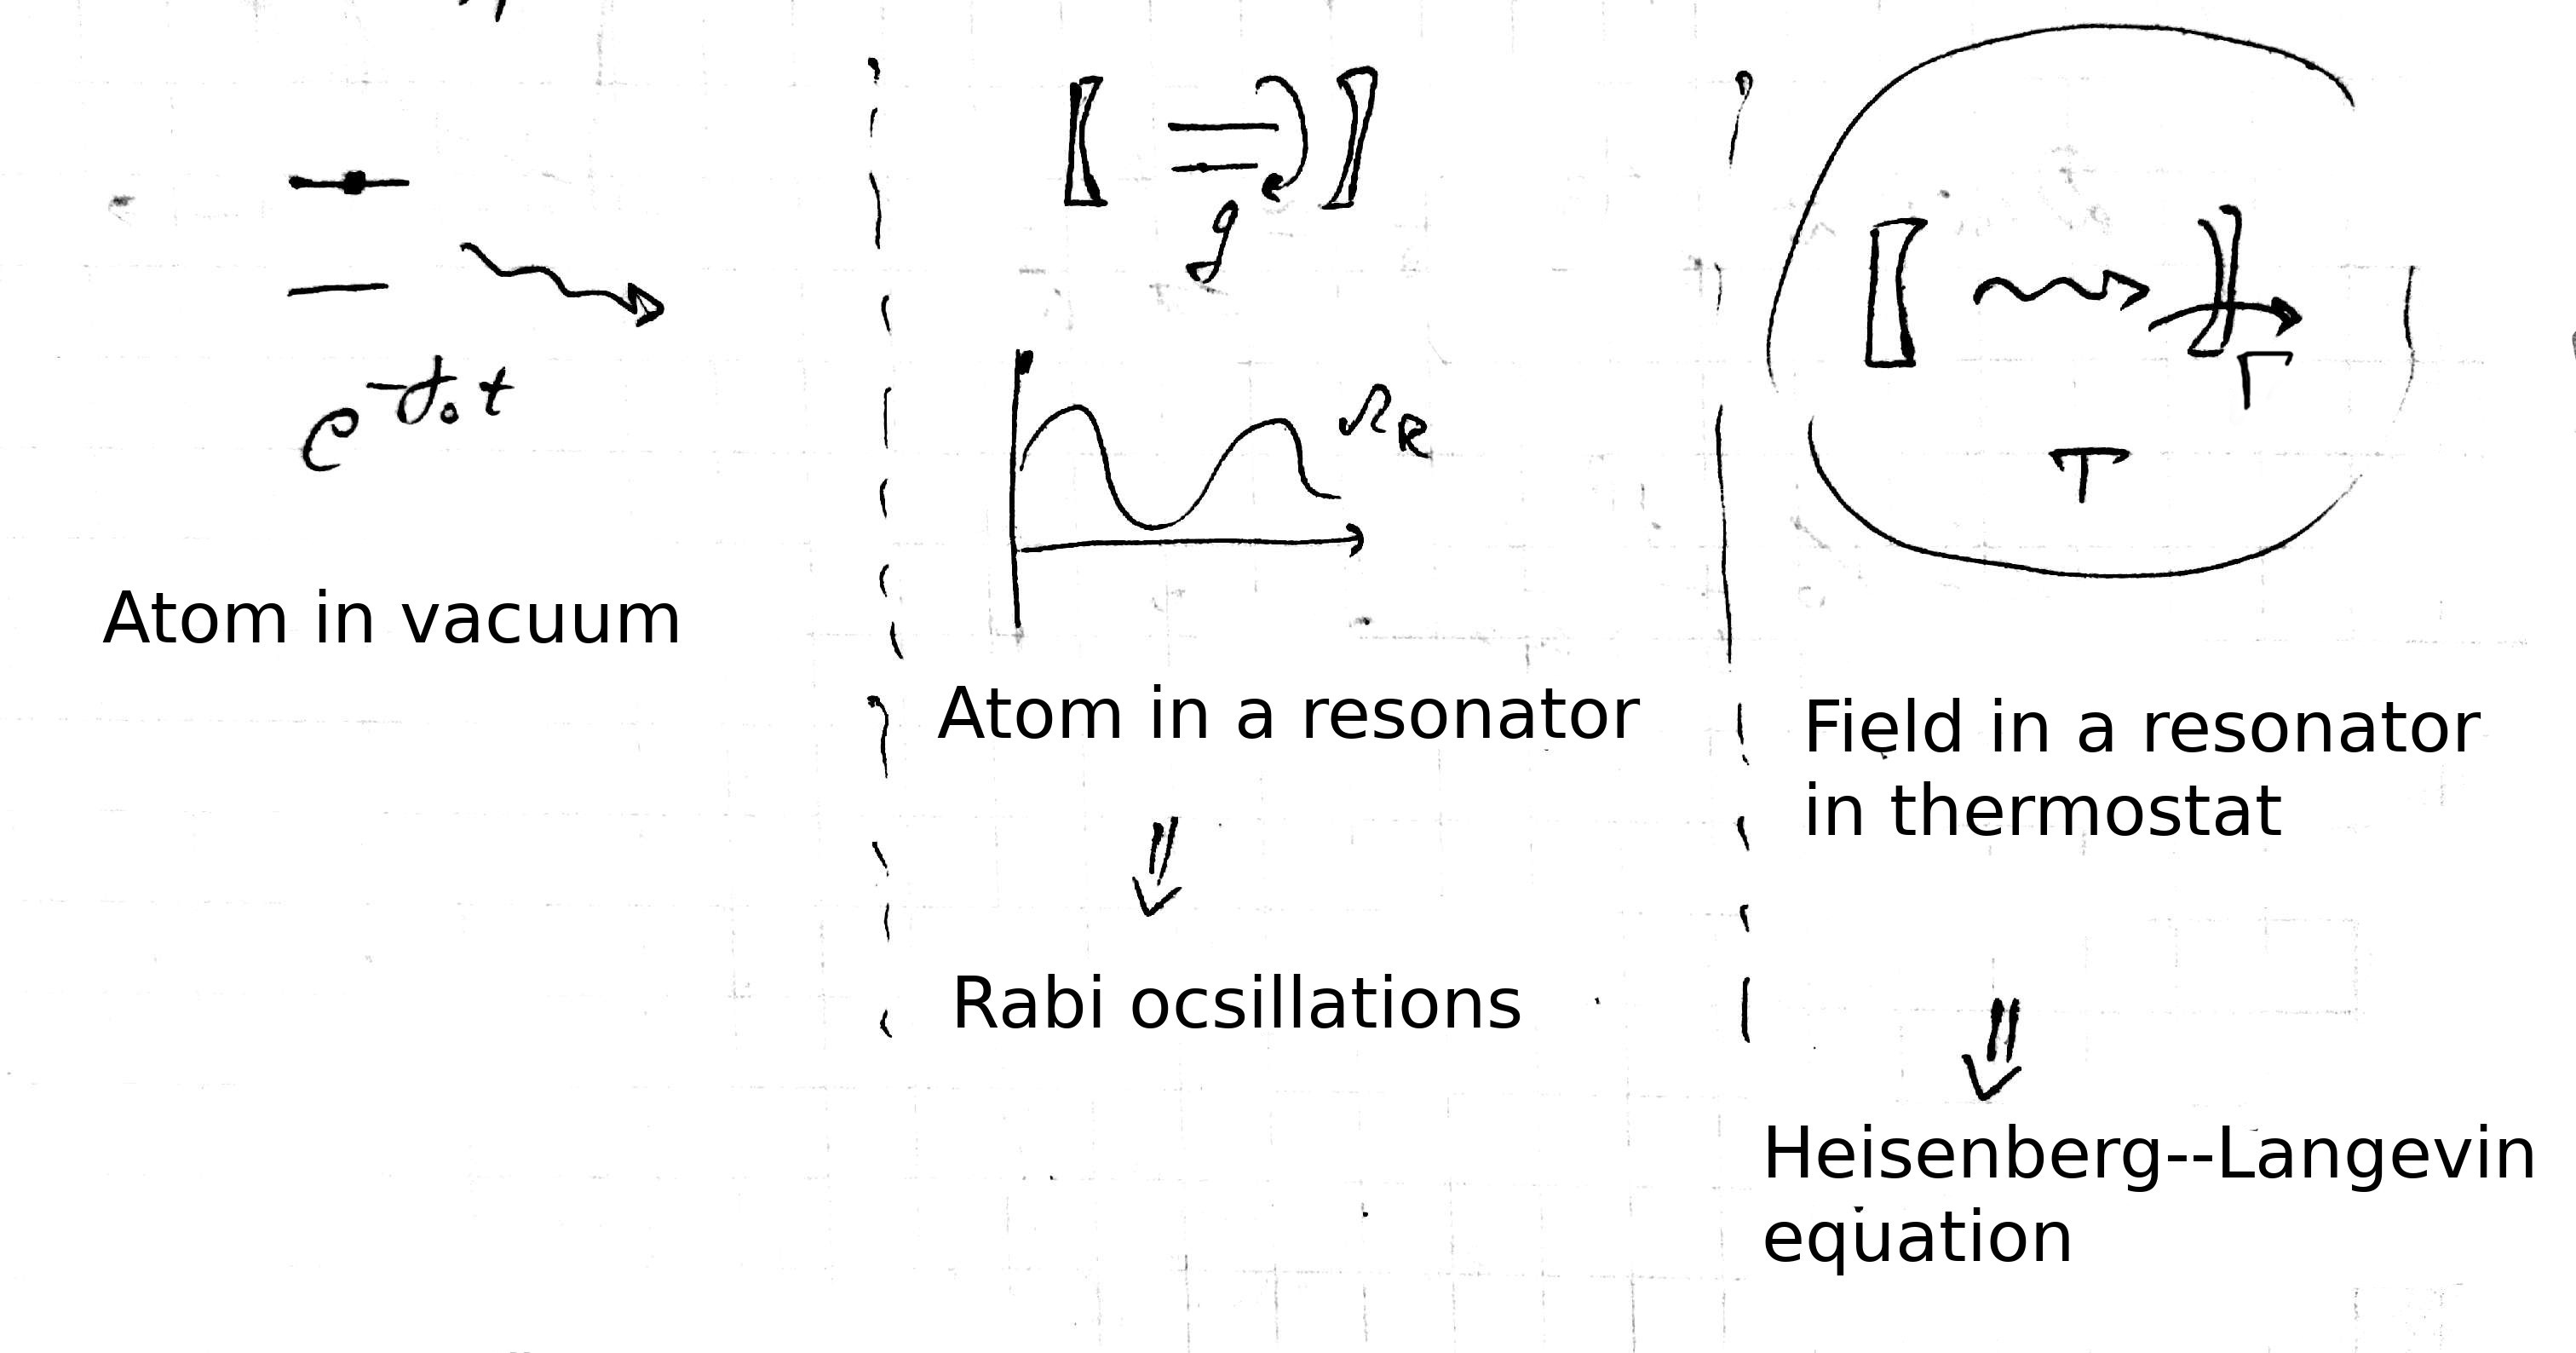
\includegraphics[width=0.7\linewidth]{fig/L10/before}
	\caption{From left to right: atom in vacuum, atom in the cavity, field in a cavity in a thermostat.}
	\label{fig:before}
\end{figure}


Here we are going to study the evolution of a single two-level atom initially prepared in the upper level $\ket{a}$ of the transition resonant with the cavity mode (fig \ref{fig:atominr}). In particular, it is seen that the spontaneous emission rate of the atom inside a resonant cavity is substantially enhanced over its free-space value (Purcell effect).

\begin{figure}[h!]
	\centering
	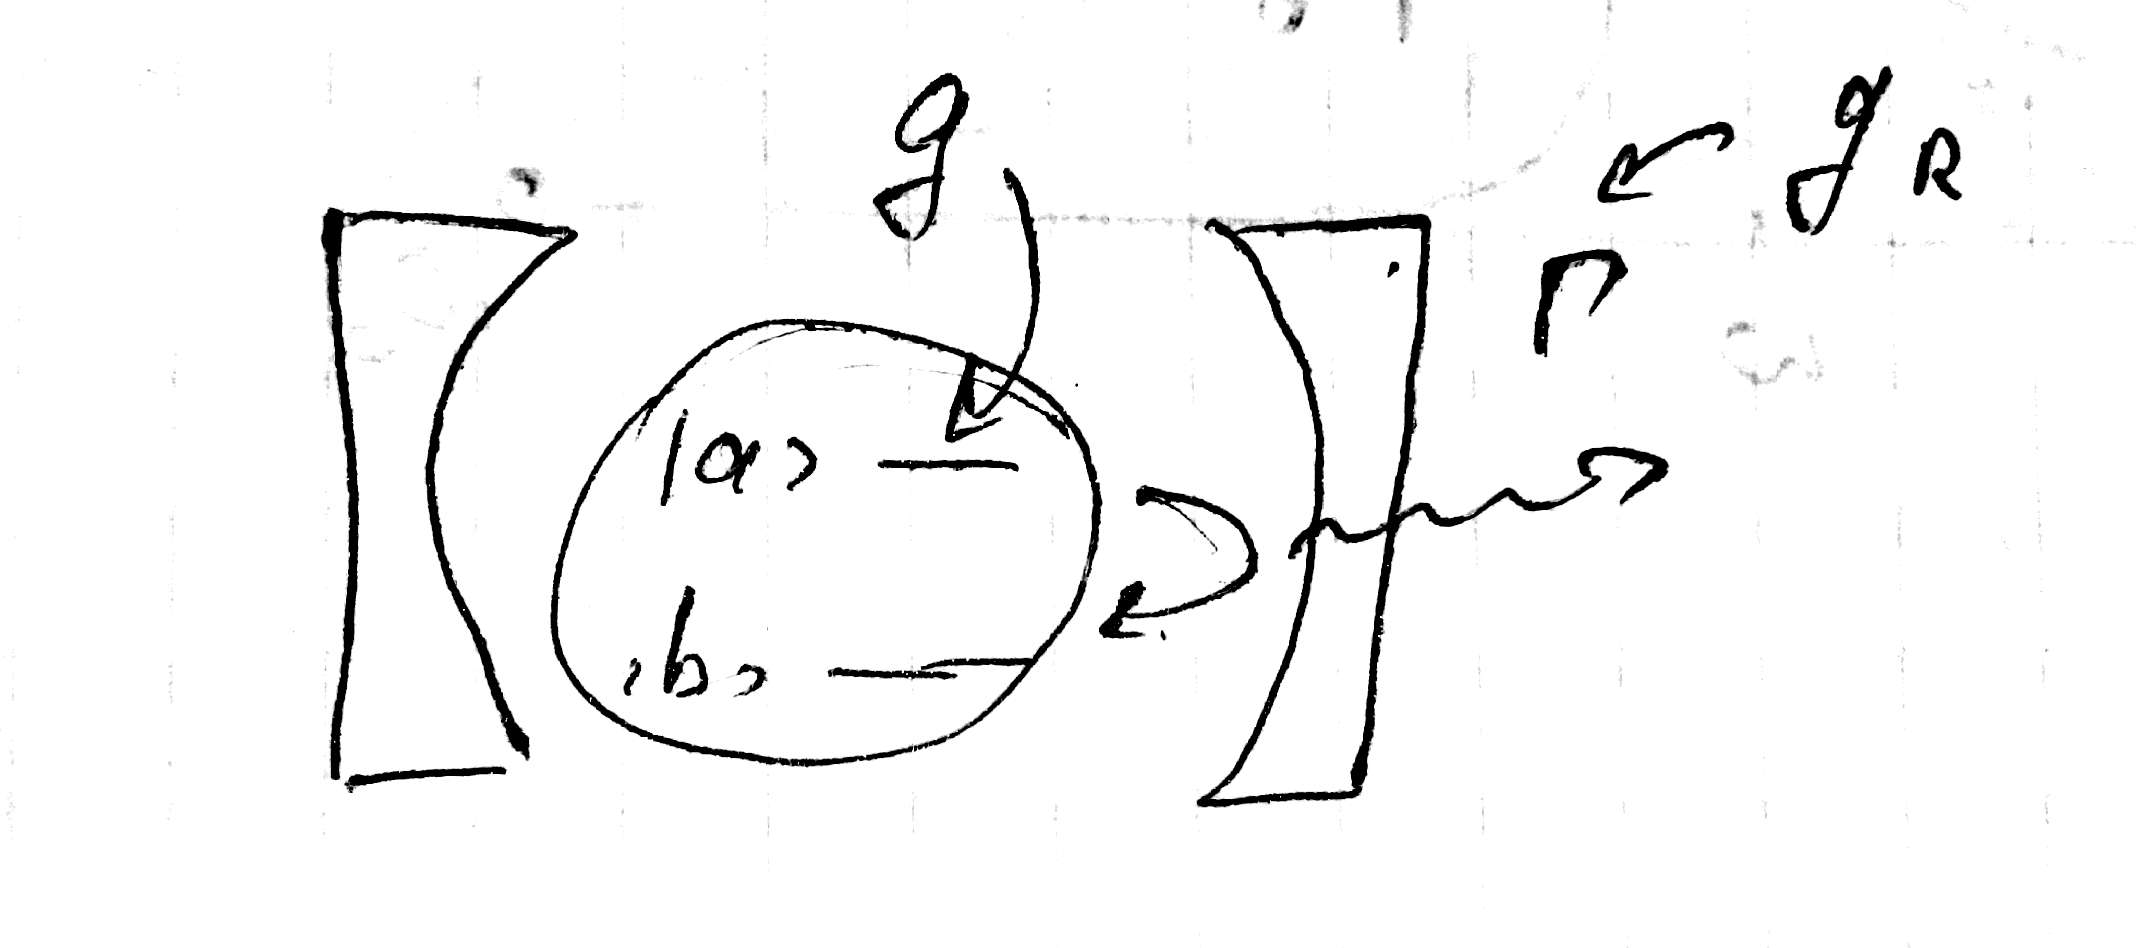
\includegraphics[width=0.3\linewidth]{fig/L10/atom_in_R}
	\caption{Atom in a cavity with losses. System has two coupling constants: $g$ --- atom and field coupling, $\Gamma$ --- cavity and reservoir coupling (transparency of a mirror)}
	\label{fig:atominr}
\end{figure}

\subsection{The Purcell factor for a closed cavity}

The decay rate $\gamma$ can be written as
\begin{equation}
	\gamma = 2 \pi \left| g(\omega) \right|^2 \frac{D(\omega)}{V},
	\label{eq:gamma}
\end{equation}
where $\rho = D/V$ is the density of state. In vacuum it is $D_0(\omega) = \frac{\omega^2}{\pi^2 c^3}$ but in a cavity it can be approximated by the Lorentzian (fig) with resonant frequency $\omega_0$
\begin{equation}
	D(\omega) = \frac{1}{\pi} \frac{\omega_{0}/2Q}{(\omega - \omega_{0})^2 + \left( \omega_{0}/2Q \right)^2}.
\end{equation}

\begin{figure}
	\centering
	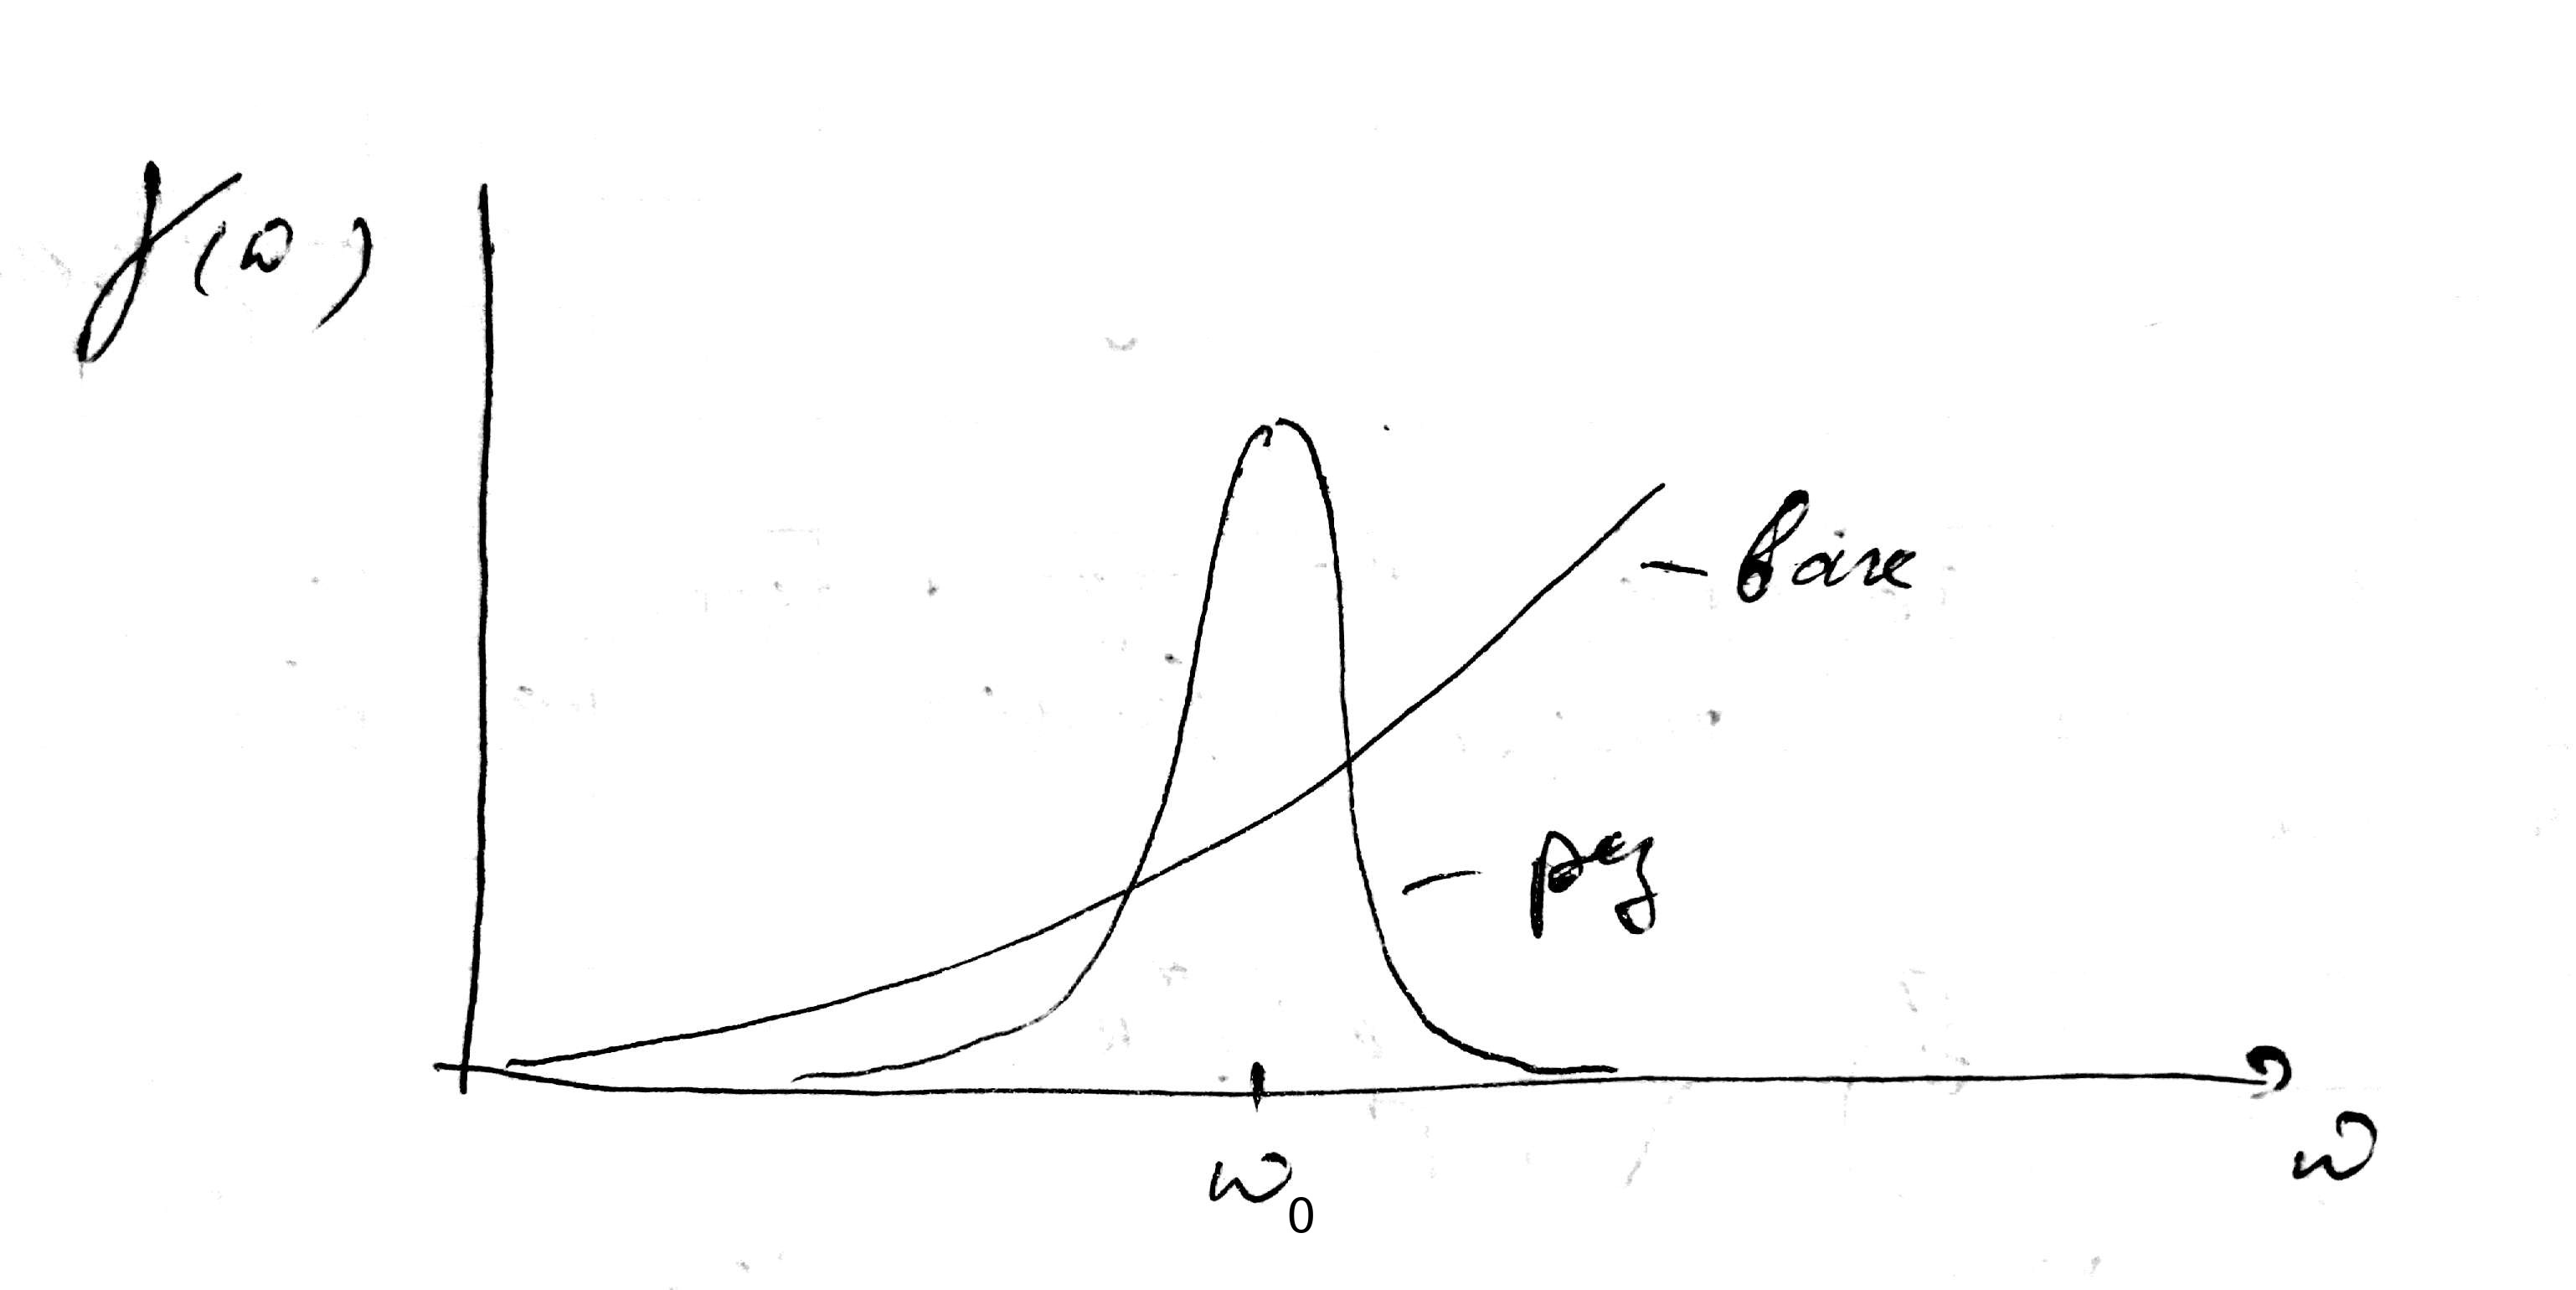
\includegraphics[width=0.5\linewidth]{fig/L10/gamma}
	\caption{The decay rate in vacuum and in a cavity}
	\label{fig:gamma}
\end{figure}

There two cases which is interesting to consider:
\begin{enumerate}
	\item[\textit{Case 1.}] $\omega \approx \omega_0$ --- transition and cavity frequencies are approximately equal. Then
	\begin{equation}
		D(\omega = \omega_0) \approx \frac{1}{\pi} \frac{2Q}{\omega_0}.
	\end{equation}
	Substitution to \eqref{eq:gamma} gives
	\begin{equation}
		\gamma = 2\pi \left| g(\omega) \right|^2 \frac{2Q}{\pi \omega} \frac{1}{V} = \underbrace{2\pi \left| g(\omega) \right|^2 \frac{\omega^2}{\pi^2 c^3}}_{\hookrightarrow=\gamma_0} \cdot \frac{1}{V} \frac{\pi^2 c^3}{\omega^2} \cdot \frac{2Q}{\pi \omega} = \gamma_0 \frac{1}{\left(2\pi\right)^2} \frac{\lambda^3}{V} Q,
	\end{equation}
	so the Purcell factor for a cavity is strongly depends on the $\lambda^3/V$ and the quality factor $Q$:
	\begin{equation}
		\boxed{F_{\text{P}} = \frac{\gamma}{\gamma_0} = \frac{1}{\left(2\pi\right)^2} \cdot \frac{\lambda^3}{V} Q.}
	\end{equation}
	
	\item[\textit{Case 2.}] $\left|\omega_0 - \omega\right| \gg \Gamma = \omega_0 / Q$. In this case we have
	\begin{equation}
		D(\omega) \approx \frac{1}{\pi} \frac{\Gamma}{2 \omega^2} = \frac{1}{2\pi} \frac{1}{Q \omega},
	\end{equation}
	then
	\begin{equation}
		F_{\text{P}} = \frac{\gamma}{\gamma_0} = \frac{1}{\left(2\pi\right)^2} \frac{\lambda^3}{V} \cdot \frac{1}{Q}.
	\end{equation}
	Usually $Q \gg 1$ and $\frac{\lambda^3}{V} \sim 1$, so far from the resonance $F_{\text{P}} \ll 1$.
\end{enumerate}

\subsection{Rigorous derivation of the atomic decay}

If the approach is rigorous then we have to call Mr. Hamiltonian immediately
\begin{equation}
	\hat{\mathcal{H}} = \hat{\mathcal{H}}_{\text{A}} + \hat{\mathcal{H}}_{\text{F}} + \hat{\mathcal{H}}_{\text{AF}} + \hat{\mathcal{H}}_{\text{R}} + \hat{\mathcal{H}}_{\text{RF}},
\end{equation}
where A stands for atom, F for field and R for reservoir. Summands of $\hat{\mathcal{H}}$ are the following
\begin{equation}
	\hat{\mathcal{H}}_{\text{F}} = \hbar \omega \hat{n}, \qquad \hat{\mathcal{H}}_{\text{A}} = \half \hbar \omega_0 \hat{\sigma}_z, \qquad \hat{\mathcal{H}}_{\text{R}} = \sum_{\kv} \hbar \omega_{\kv} \hat{n}_{\kv},
\end{equation}
\begin{equation}
	\hat{\mathcal{H}}_{\text{AF}} = \hbar g \left( \hat{\sigma}_+ \hat{a} + \hat{a}^{\dagger} \hat{\sigma}_- \right),  \qquad \hat{\mathcal{H}}_{\text{FR}} = \hbar \sum_{\kv} g_{\kv} \left( \hat{a}^{\dagger} \hat{b}_{\kv} +  \hat{b}^{\dagger}_{\kv} \hat{a} \right), \qquad 
	g, g_{\kv} \in \mathbb{R}.
\end{equation}

We are interested in time dependence of $\av{\hat{\sigma}_z}$ and $\av{\hat{a}^{\dagger} \hat{a}}$. Angle brackets represents the averaging over the reservoir and quantum mechanics averaging $\av{\dots} \equiv \av{\av{\dots}_{\text{R}}}_{\text{QM}}$. For an any atom operator $\hat{O}_{\text{A}}$ we have a supporting relation
\begin{equation}
	\frac{d}{dt} \av{(\hat{a}^{\dagger})^m (\hat{a})^n \hat{O}_{\text{A}} }= - \frac{i}{\hbar} \left[ (\hat{a}^{\dagger})^m (\hat{a})^n \hat{O}_{\text{A}}, \hat{\mathcal{H}}_{\text{A}} + \hat{\mathcal{H}}_{\text{F}} + \hat{\mathcal{H}}_{\text{AF}} \right] + \frac{d}{dt} \av{ (\hat{a}^{\dagger})^m (\hat{a})^n } \hat{O}_{\text{A}}.
\end{equation} 
Similar to \eqref{eq:dn} it is not so hard to obtain the answer for a any positive integer powers 
\begin{multline}
	\frac{d}{dt} \av{(\hat{a}^{\dagger})^m (\hat{a})^n} = \left[ i \omega (m-n) - \frac{\Gamma}{2}(m+n) \right] \av{(\hat{a}^{\dagger})^m (\hat{a})^n} + \\ + \Gamma\cdot  mn \cdot \bar{\hat{n}}_{\text{R}} \av{(\hat{a}^{\dagger})^{m-1} (\hat{a})^{n-1}}.
\end{multline}
In the particular case, when $\hat{O}_{\text{A}} = \hat{\mathbb{1}}$, we have
\begin{equation}
	\frac{d}{dt} \av{\hat{a}^{\dagger} \hat{a}} = - \frac{i}{\hbar} \av{\left[ \hat{a}^{\dagger} \hat{a}, \hat{\mathcal{H}}_{\text{A}} + \hat{\mathcal{H}}_{\text{F}} + \hat{\mathcal{H}}_{\text{AF}} \right]} - \Gamma \av{\hat{a}^{\dagger} \hat{a}} + \Gamma \bar{\hat{n}}_{\text{R}}.
\end{equation}
As the commutator of $\hat{a}$ is trivial $\left[\hat{a}, \hat{a}^{\dagger}\right]=1$, so
\begin{equation}
	\left[ \hat{a}^{\dagger} \hat{a}, g \left( \hat{\sigma}_+ \hat{a} + \hat{a}\dag \hat{\sigma}_-\right) \right] =  g \hat{a}\dag \hat{\sigma}_- - g \hat{\sigma}_+ \hat{a},
\end{equation}
then
\begin{equation}
	\frac{d}{dt} \av{\hat{a}^{\dagger} \hat{a}} = - \frac{i}{\hbar} g\underbrace{\av{\hat{a}\dag \hat{\sigma}_- - \hat{\sigma}_+ \hat{a}}}_{?} - \Gamma \av{\hat{a}^{\dagger} \hat{a}} + \Gamma \bar{\hat{n}}_{\text{R}},
	\label{eq:aa}
\end{equation}
where $\av{\hat{a}\dag \hat{\sigma}_- - \hat{\sigma}_+ \hat{a}}$ is yet unknown.

Now let us take a look at sigma--$z$ operator
\begin{equation}
	\frac{d}{dt} \av{\hat{\sigma}_z} = -\frac{i}{\hbar} \av{\left[ \hat{\sigma}_z, g \hat{a}\dag \hat{\sigma}_- + g \hat{\sigma}_+ \hat{a} \right]} = 2 g\frac{i}{\hbar} \underbrace{\av{\hat{a}\dag \hat{\sigma}_- - \hat{\sigma}_+ \hat{a}}}_{?},
	\label{eq:sigmaz}
\end{equation}
where we have got the same unknown averaging. To obtain last result the commutation relations for $\sigma$--matrices had been used:
\begin{equation}
	\left[ \hat{\sigma}_z, \hat{\sigma}_- \right] = - 2 \hat{\sigma}_-, \qquad
	\left[ \hat{\sigma}_z, \hat{\sigma}_+ \right] = 2 \hat{\sigma}_+.
\end{equation}

To solve \eqref{eq:aa} and \eqref{eq:sigmaz} we need to know the time dependence of that unknown Hermitean operator $\av{\hat{a}\dag \hat{\sigma}_- - \hat{\sigma}_+ \hat{a}}$, which equation of motion involves the quantity $\av{\hat{a}\dag \hat{\sigma}_z \hat{a}}$ and so on. In general, we get an infinite set of equations which may not be analytically solvable. The way out is the following --- we need to cut the chain of equations at some step. Here the things we are going to suppose:
\begin{enumerate}
	\item Put cavity at zero temperature reservoir ($\bar{\hat{n}}_{\text{R}} = 0$).
	\item Initially the atom is in the excited sate $\ket{a}$ and field inside the cavity is in the vacuum state $\ket{0}$.
\end{enumerate}
In other words, we consider \textit{a single photon approximation}. If the photon is only one then all summands which are proportional to $\hat{a}^2$ or $\hat{a}^{\dagger 2}$ are identically zero. As the result, under these conditions, we obtain the following system of equations:
\begin{equation}
	\begin{cases}
		\frac{d}{dt} \av{\hat{a}\dagger\hat{a}} = g \chi(t) - \Gamma \av{\hat{a}\dagger\hat{a}} \\
		\frac{d}{dt} \av{\hat{\sigma}_z} = - 2 g \chi(t) \\
		\frac{d}{dt} \chi(t) = g \av{\hat{\sigma}_z} + 2 g \cdot y(t) + g - \frac{\Gamma}{2} \chi(t) \\
		\frac{d}{dt} y(t) = - g \chi(t) - \Gamma y(t)
	\end{cases},
	\qquad 
	\begin{matrix}
		\chi(t) &\myeq& i \av{\hat{\sigma}_+ \hat{a} - \hat{a}\dag\hat{\sigma}_-}, \\
		y(t) &\myeq& \av{\hat{a}\dagger\hat{\sigma}_z \hat{a}}, \qquad \quad \ 
	\end{matrix}
\end{equation}
with the initial conditions 
\begin{equation}
	\chi \big|_{t=0} = 0, \qquad y \big|_{t=0} = 0, \qquad \av{\hat{a}\dag\hat{a}} \big|_{t=0} = 0, \qquad \av{\hat{\sigma}_z} \big|_{t=0} = 1. 
\end{equation}

Using the single photon approximation is always simplifies the problem and make it look more "classical".

This system has two main parameters: $g$ and $\Gamma$ (see fig. \ref{fig:atominr}). Let us consider two limiting behavior regimes:
\begin{enumerate}
	\item[\textit{Regime 1.}] $\Gamma \gg g \to \Gamma \gg \Omega_R$ or a  \textit{overdamping} regime. Here we have
	\begin{equation}
		\av{\hat{\sigma}_z} = -1 + 2 e^{-4 g^2 \frac{t}{\Gamma}} = - 1 + 2e^{- \gamma t},
	\end{equation}
	where 
	\begin{equation}
		\gamma = \frac{4 g^2}{\Gamma} = \frac{4 g^2 Q}{\omega} = \underbrace{\frac{6\pi c^3 Q}{V \omega^2}}_{F_{\text{P}}} \cdot \frac{8 \left|\vec{d}\right|^2 \omega^2}{\hbar \omega_0 c^3} \quad \to \quad \gamma \sim F_{\text{P}}.
	\end{equation}
	The cavity increase the dissipation rate!
	\item[\textit{Regime 2.}] $\Gamma \ll g$ or a \textit{low losses} regime. Here we can obtain that the atomic inversion $\av{\hat{\sigma}_z}$ is
	\begin{equation}
		\av{\hat{\sigma}_z} = - 1 + e^{- \frac{\Gamma}{2} t} \left[1 + \cos \left( 2 gt \right)\right]
	\end{equation}
	so the probability $P_a$ take the simple form
	\begin{equation}
		P_a = \av{\hat{\sigma}_z} + 1 = e^{- \frac{\Gamma}{2} t} \left[1 + \cos \left( 2 gt \right)\right]
	\end{equation}
\end{enumerate}
Different regimes are represented on a fig. \ref{fig:regimes}.

\begin{figure}
	\centering
	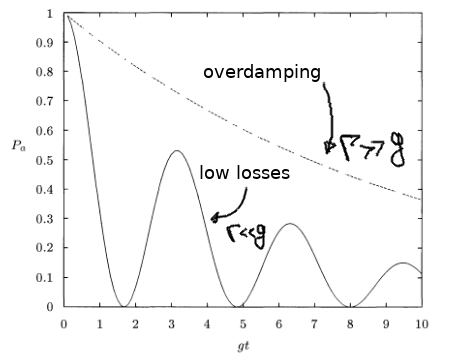
\includegraphics[width=0.7\linewidth]{fig/L10/regimes}
	\caption{Probability $P_a$ versus dimensionless time $gt$ for the different limiting behavior regimes.}
	\label{fig:regimes}
\end{figure}
